\documentclass{article}

\usepackage{amsmath}
\usepackage{hyperref}
\usepackage{graphicx}
\usepackage{float}
\usepackage{tikz}
    \usetikzlibrary{backgrounds,fit,positioning,calc}
    \pgfdeclarelayer{background}
    \pgfdeclarelayer{backbackground}
    \pgfsetlayers{backbackground,background,main}
    \tikzset{
        framed,
        node distance=3mm,
        layer/.style={rectangle, draw=black, font=\fontsize{6}{6}\selectfont, fill=cyan!30},
        sum/.style={circle, draw=black, font=\fontsize{6}{6}\selectfont, fill=red!30, inner sep=1pt},
        annot/.style={font=\fontsize{6}{6}\selectfont}
    }

\title{Predictiing the binding between zinc-finger protein and DNA}

\author{
    Li, Tianjie\\
    \texttt{zacharylee.cn@gmail.com}
    \and
    Li, Jingwei\\
    \texttt{ljw2017@sjtu.edu.cn}
    \and
    Wu, Qiang\\
    \texttt{qiangwu@sjtu.edu.cn}
}

\date{\today}

\begin{document}

\maketitle

\section{Methods}

\subsection{Process mouse C2H2 zinc finger protein data}
We search the C2H2 zinc finger protein for mouse on uniprot with the query (ft\_zn\_fing:C2H2) AND (organism\_name:``Mus musculus''). Totally 380 proteins are returned and downloaded. We also download the corresponding 3D structures of the 380 proteins from alphafoldDB. We filter 6 proteins without 3D structures and 4 proteins with inconsistent sequence lengths on uniprot and alphafoldDB. We then convert protein 3D structures to secondary structures by dssp\cite{10.1093/nar/gkq1105}, which predicts 9 secondary structures:
\begin{description}
    \item[H] $\alpha$-helix.
    \item[B] Residue in isolated $\beta$-bridge.
    \item[E] Extended strand participating in $\beta$ ladder.
    \item[G] 310-helix.
    \item[I] $\pi$-helix.
    \item[P] $\kappa$-helix (poly-proline II helix).
    \item[T] Hydrogen-bonded turn.
    \item[S] Bend.
    \item[-] None.
\end{description}
Since C2H2 zinc fingers are important for protein binding, we mark them as additional secondary structure Z. Also, KRAB is quite common in C2H2 zinc fingers. We mark them as additional secondary structure K. Totally 370 C2H2 zinc finger proteins of mouse are piped for downsteam analyses.

\subsection{Process ChIP-seq data}
Among the 370 zinc finger proteins of mouse, only 62 proteins have ChIP-seq data on ncbi. We download these raw ChIP-seq data and map them to mm9 genome assembly by bowtie2 and call peaks by macs3. We filter out peaks intersect the black list in \url{http://mitra.stanford.edu/kundaje/akundaje/release/blacklists/mm9-mouse/mm9-blacklist.bed.gz}. Peaks with at least 50-bp overlapping are clustered together. For each cluster, we only select a single peak whose p-pvalue is quantiled at 90\%. We avoid the peaks with highest p-values in clusters because those peaks may be repeated loci or other false positive peaks. To control the peak size, the widest 10\% peaks and the narrowest 10\% peaks are filtered. To further decrease the proportion of false positive peaks, we filter the 10\% peaks with the highest and lowest p-values. To save the training time, we randomly select 3000 survive peaks for each protein and extract 100-bp sequences at peak summits.

\subsection{Tokenize}

We use m to represents mask token to pad DNA of different lengths to the same length at end. Resembling BERT\cite{devlin-etal-2019-bert}, we use c to represent a classification token and pad it add the start of DNA. The embedding of the classification token output by the transformer structure is input to the classification header to get the final logits. The vocabulary of DNA is thus mcACGTN, which is tokenized to 0-6.

We use ProteinBert to encode the protein sequence, which uses a specific token p to pad protein of different lengths to the same length at end\cite{10.1093/bioinformatics/btac020}. ProteinBert also include a start token s and an end token e at the start and end of the protein sequence respectively to indicate the actual length of the protein sequence. Besides the 20 common amino acids, ProteinBert use U to represent selenocysteine, X to represent undefined amino-acid, and o to represent other amino acids. The vocalulary of protein is thus ACDEFGHIKLMNPQRSTUVWXYosep, which is tokenized to 0-25.

The secondary structure has the same length as protein. We encode secondary structure by a strand transformer encoder module. Like DNA, we use mask token to pad secondary structures of different lengths to the same length at end. Besides the 9 secondary structure predicted by dssp, we also represent C2H2 zinc finger by Z and KRAB by K. The vocalulary of secondary structure is thus mHBEGIPTS-KZ, which is tokenized to 0-11.

\subsection{AI models}

\subsubsection{Full architecture}

The full architecture of our model is given in Fig. \ref{fig:full_architecture}. It consists of four parts.
\begin{enumerate}
    \item A self-attention module of DNA embeddings.
    \item A cross-attention module between DNA embeddings and protein embeddings.
    \item A cross-attention module between DNA embeddings and secondary structure embeddings.
    \item A feedforward module.
    \item A classifier module.
\end{enumerate}
The input DNA sequence is tokenized and embedded to a dimention of 128. The DNA embedding is piped to a self-attention module with residual structure. Resembling DeepSeek\cite{deepseekai2024deepseekv2strongeconomicalefficient}, we use RMS normalization to replace layer normalization, and move the normalization before self- and cross- attention modules. We use the multi-head attention module implemented in torchtune. The rotary positional embeddings (RoPE) is included in the implemention in torchtune\cite{SU2024127063}, and is applied only to query and key embeddings, but not value embeddings. The torchtune implementation also contains an output linear projection module.

Only the outout embedding of classification token of DNA self-attention is passed to the downstream cross-attention module to be projected to query embeddings. The cross-attention also take the protein embeddings as input, which is generated by ProteinBert. The protein embeddings are to be projected to key and value embeddings. The output embeddings of the DNA-protein cross-attention module is further passed to the secondary-DNA cross-attention module. This time, the key and value embeddings is generated by the secondary structure embeddings. The secondary structure embeddings contain the information of C2H2 zinc fingers, and is generated by a strandard self-attention transformer encoder.

The output embeddings of the secondary-DNA cross-attention module is piped to the feedforward network. The DNA self-attention module, the DNA-protein cross-attention module, the secondary-DNA cross-attention module and the feedforward network module are repeated by several times. The final output embedding of the classification token of DNA is then normalized and passed to the classifer header to get the final logit outputs.

Our model encode DNA, protein and secondary structure respectively, and then use cross-attention to flow information from protein and secondary structure to DNA. We do transfer learning based on the pre-trained ProteinBert model, which generally performs better than de novo training.

\begin{figure}[H]
    \centering
    \makebox[0pt]{
        \hspace*{0cm}

        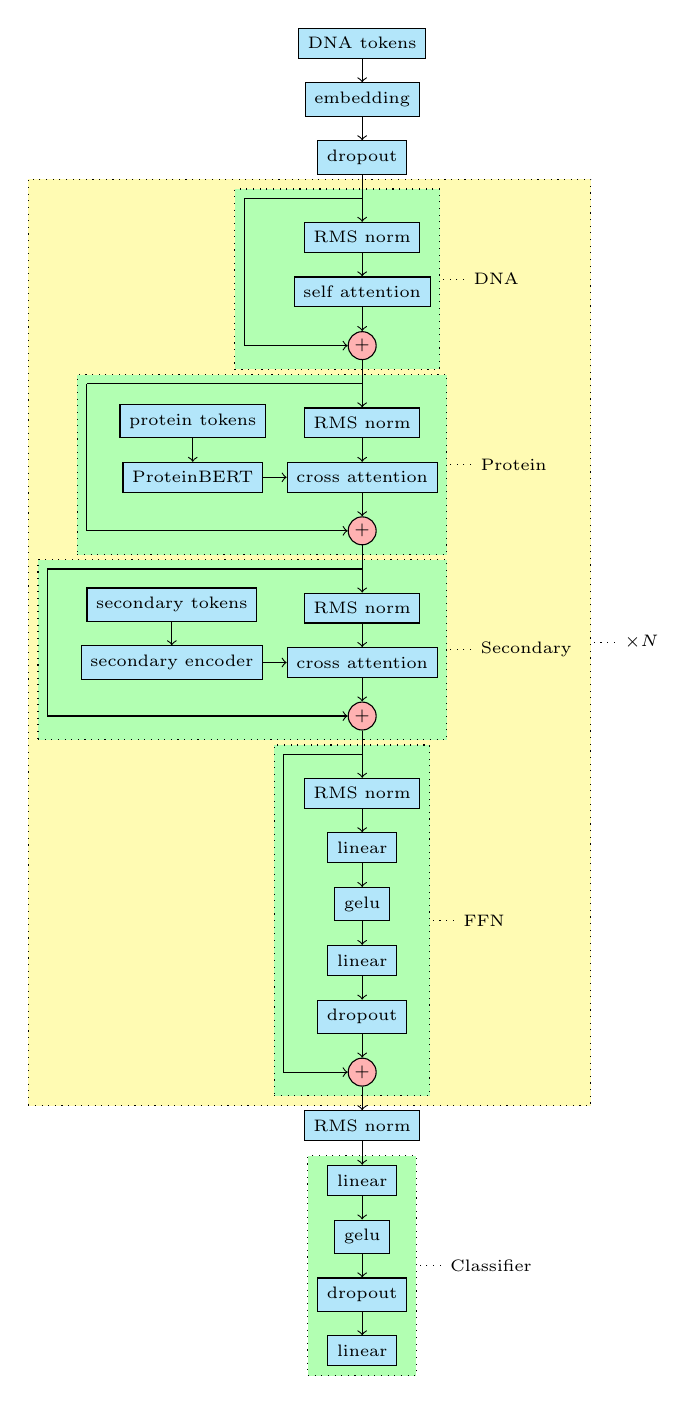
\begin{tikzpicture}
            \node[layer] (DNAToken) {DNA tokens};
            \node[layer] (Embed) [below=of DNAToken] {embedding};
            \draw[->] (DNAToken) -- (Embed);
            \node[layer] (EmbedDrop) [below=of Embed] {dropout};
            \draw[->] (Embed) -- (EmbedDrop);

            \coordinate[below=of EmbedDrop] (SelfResidualStart);
            \draw[-] (EmbedDrop) -- (SelfResidualStart);
            \node[layer] (SelfNormRMS) [below=of SelfResidualStart] {RMS norm};
            \draw[->] (SelfResidualStart) -- (SelfNormRMS);
            \node[layer] (SelfAttention) [below=of SelfNormRMS] {self attention};
            \draw[->] (SelfNormRMS) -- (SelfAttention);
            \node[sum] (SelfResidualEnd) [below=of SelfAttention] {$+$};
            \draw[->] (SelfAttention) -- (SelfResidualEnd);

            \coordinate[left=1.5cm of SelfResidualStart.center] (SelfResidualStartAnchor);
            \coordinate[left=1.5cm of SelfResidualEnd.center] (SelfResidualEndAnchor);
            \draw[-] (SelfResidualStart) -- (SelfResidualStartAnchor);
            \draw[-] (SelfResidualStartAnchor) -- (SelfResidualEndAnchor);
            \draw[->] (SelfResidualEndAnchor) -- (SelfResidualEnd);

            \begin{pgfonlayer}{background}
                \node[draw, dotted, fill=green!30, fit=(SelfResidualStart)(SelfNormRMS)(SelfAttention)(SelfResidualEnd)(SelfResidualStartAnchor)(SelfResidualEndAnchor)] (DNAModule) {};
                \node[annot] (DNAModuleName) [right=of DNAModule] {DNA};
                \draw[dotted] (DNAModuleName) -- (DNAModule);
            \end{pgfonlayer}

            \coordinate[below=of SelfResidualEnd] (ProteinResidualStart);
            \draw[-] (SelfResidualEnd) -- (ProteinResidualStart);
            \node[layer] (ProteinNormRMS) [below=of ProteinResidualStart] {RMS norm};
            \draw[->] (ProteinResidualStart) -- (ProteinNormRMS);
            \node[layer] (ProteinAttention) [below=of ProteinNormRMS] {cross attention};
            \draw[->] (ProteinNormRMS) -- (ProteinAttention);            
            \node[sum] (ProteinResidualEnd) [below=of ProteinAttention] {$+$};
            \draw[->] (ProteinAttention) -- (ProteinResidualEnd);

            \coordinate[left=3.5cm of ProteinResidualStart.center] (ProteinResidualStartAnchor);
            \coordinate[left=3.5cm of ProteinResidualEnd.center] (ProteinResidualEndAnchor);
            \draw[-] (ProteinResidualStart) -- (ProteinResidualStartAnchor);
            \draw[-] (ProteinResidualStartAnchor) -- (ProteinResidualEndAnchor);
            \draw[->] (ProteinResidualEndAnchor) -- (ProteinResidualEnd);

            \node[layer] (ProteinBERT) [left=of ProteinAttention] {ProteinBERT};
            \draw[->] (ProteinBERT) -- (ProteinAttention);
            \node[layer] (ProteinToken) [above=of ProteinBERT] {protein tokens};
            \draw[->] (ProteinToken) -- (ProteinBERT);

            \begin{pgfonlayer}{background}
                \node[draw, dotted, fill=green!30, fit=(ProteinResidualStart)(ProteinNormRMS)(ProteinAttention)(ProteinResidualEnd)(ProteinResidualStartAnchor)(ProteinResidualEndAnchor)(ProteinBERT)(ProteinToken)] (ProteinModule) {};
                \node[annot] (ProteinModuleName) [right=of ProteinModule] {Protein};
                \draw[dotted] (ProteinModuleName) -- (ProteinModule);
            \end{pgfonlayer}

            \coordinate[below=of ProteinResidualEnd] (SecondResidualStart);
            \draw[-] (ProteinResidualEnd) -- (SecondResidualStart);
            \node[layer] (SecondNormRMS) [below=of SecondResidualStart] {RMS norm};
            \draw[->] (SecondResidualStart) -- (SecondNormRMS);
            \node[layer] (SecondAttention) [below=of SecondNormRMS] {cross attention};
            \draw[->] (SecondNormRMS) -- (SecondAttention);
            \node[sum] (SecondResidualEnd) [below=of SecondAttention] {$+$};
            \draw[->] (SecondAttention) -- (SecondResidualEnd);

            \coordinate[left=4cm of SecondResidualStart.center] (SecondResidualStartAnchor);
            \coordinate[left=4cm of SecondResidualEnd.center] (SecondResidualEndAnchor);
            \draw[-] (SecondResidualStart) -- (SecondResidualStartAnchor);
            \draw[-] (SecondResidualStartAnchor) -- (SecondResidualEndAnchor);
            \draw[->] (SecondResidualEndAnchor) -- (SecondResidualEnd);

            \node[layer] (SecondEncoder) [left=of SecondAttention] {secondary encoder};
            \draw[->] (SecondEncoder) -- (SecondAttention);
            \node[layer] (SecondToken) [above=of SecondEncoder] {secondary tokens};
            \draw[->] (SecondToken) -- (SecondEncoder);

            \begin{pgfonlayer}{background}
                \node[draw, dotted, fill=green!30, fit=(SecondResidualStart)(SecondNormRMS)(SecondAttention)(SecondResidualEnd)(SecondResidualStartAnchor)(SecondResidualEndAnchor)(SecondEncoder)(SecondToken)] (SecondModule) {};
                \node[annot] (SecondModuleName) [right=of SecondModule] {Secondary};
                \draw[dotted] (SecondModuleName) -- (SecondModule);
            \end{pgfonlayer}

            \coordinate[below=of SecondResidualEnd] (FFNResidualStart);
            \draw[-] (SecondResidualEnd) -- (FFNResidualStart);
            \node[layer] (FNNNormRMS) [below=of FFNResidualStart] {RMS norm};
            \draw[->] (FFNResidualStart) -- (FNNNormRMS);
            \node[layer] (FFNLinear1) [below=of FNNNormRMS] {linear};
            \draw[->] (FNNNormRMS) -- (FFNLinear1);
            \node[layer] (FFNGelu) [below=of FFNLinear1] {gelu};
            \draw[->] (FFNLinear1) -- (FFNGelu);
            \node[layer] (FFNLinear2) [below=of FFNGelu] {linear};
            \draw[->] (FFNGelu) -- (FFNLinear2);
            \node[layer] (FFNDrop) [below=of FFNLinear2] {dropout};
            \draw[->] (FFNLinear2) -- (FFNDrop);
            \node[sum] (FFNResidualEnd) [below=of FFNDrop] {+};
            \draw[->] (FFNDrop) -- (FFNResidualEnd);

            \coordinate[left=1cm of FFNResidualStart.center] (FFNResidualStartAnchor);
            \coordinate[left=1cm of FFNResidualEnd.center] (FFNResidualEndAnchor);
            \draw[-] (FFNResidualStart) -- (FFNResidualStartAnchor);
            \draw[-] (FFNResidualStartAnchor) -- (FFNResidualEndAnchor);
            \draw[->] (FFNResidualEndAnchor) -- (FFNResidualEnd);

            \begin{pgfonlayer}{background}
                \node[draw, dotted, fill=green!30, fit=(FFNResidualStart)(FNNNormRMS)(FFNLinear1)(FFNGelu)(FFNLinear2)(FFNDrop)(FFNResidualEnd)(FFNResidualStartAnchor)(FFNResidualEndAnchor)] (FFNModule) {};
                \node[annot] (FFNModuleName) [right=of FFNModule] {FFN};
                \draw[dotted] (FFNModuleName) -- (FFNModule);
            \end{pgfonlayer}

            \begin{pgfonlayer}{backbackground}
                \node[draw, dotted, fill=yellow!30, fit=(DNAModule)(DNAModuleName)(ProteinModule)(ProteinModuleName)(SecondModule)(SecondModuleName)(FFNModule)(FFNModuleName)] (Repeats) {};
                \node[annot] (RepeatsTimesN) [right=of Repeats] {$\times N$};
                \draw[dotted] (RepeatsTimesN) -- (Repeats);
            \end{pgfonlayer}

            \node[layer] (LastNormRms) [below=of FFNResidualEnd] {RMS norm};
            \draw[->] (FFNResidualEnd) -> (LastNormRms);

            \node[layer] (CLSLinear1) [below=of LastNormRms] {linear};
            \draw[->] (LastNormRms) -- (CLSLinear1);
            \node[layer] (CLSGelu) [below=of CLSLinear1] {gelu};
            \draw[->] (CLSLinear1) -- (CLSGelu);
            \node[layer] (CLSDrop) [below=of CLSGelu] {dropout};
            \draw[->] (CLSGelu) -- (CLSDrop);
            \node[layer] (CLSLinear2) [below=of CLSDrop] {linear};
            \draw[->] (CLSDrop) -- (CLSLinear2);

            \begin{pgfonlayer}{background}
                \node[draw, dotted, fill=green!30, fit=(CLSLinear1)(CLSGelu)(CLSDrop)(CLSLinear2)] (CLSModule) {};
                \node[annot] (CLSModuleName) [right=of CLSModule] {Classifier};
                \draw[dotted] (CLSModuleName) -- (CLSModule);
            \end{pgfonlayer}
        \end{tikzpicture}
    }
    \caption{The total architecture. Apply self-attention to DNA embeddings. Then apply cross-attention with protein embeddings to the results. Further apply cross-attention with secondary structure embeddings to the results. The above process is repeated by $N$-times. The output is passed to the feedforward network and classifier header sequentially to get the final logits.}\label{fig:full_architecture}
\end{figure}

\subsubsection{ProteinBert architecture}
For completeness, we include the architecture of ProteinBert in Fig. \ref{fig:protein_bert_architecture}. It consists of several repeats of parallel global workflow handling the single global protein embedding and a local workflow handling the residue-wise embeddings. The global embedding influence the local workflow through then broadcast addition. The local embeddings influence the global workflow through the cross-attention module. The cross-attention module has linear complexity of protein length instead of quadratic because the global embedding is single. This promises the efficiency of ProteinBert even when handling long protein reads. In our case, we set the longest allowed protein sequence to be 270bp. We also add a projection header (the purple module) to process the ProteinBert output such that the embedding dimentions are consistent between ProteinBert and the remaining part of the model.

\begin{figure}[H]
    \centering
    \makebox[0pt]{
        \hspace*{0cm}

        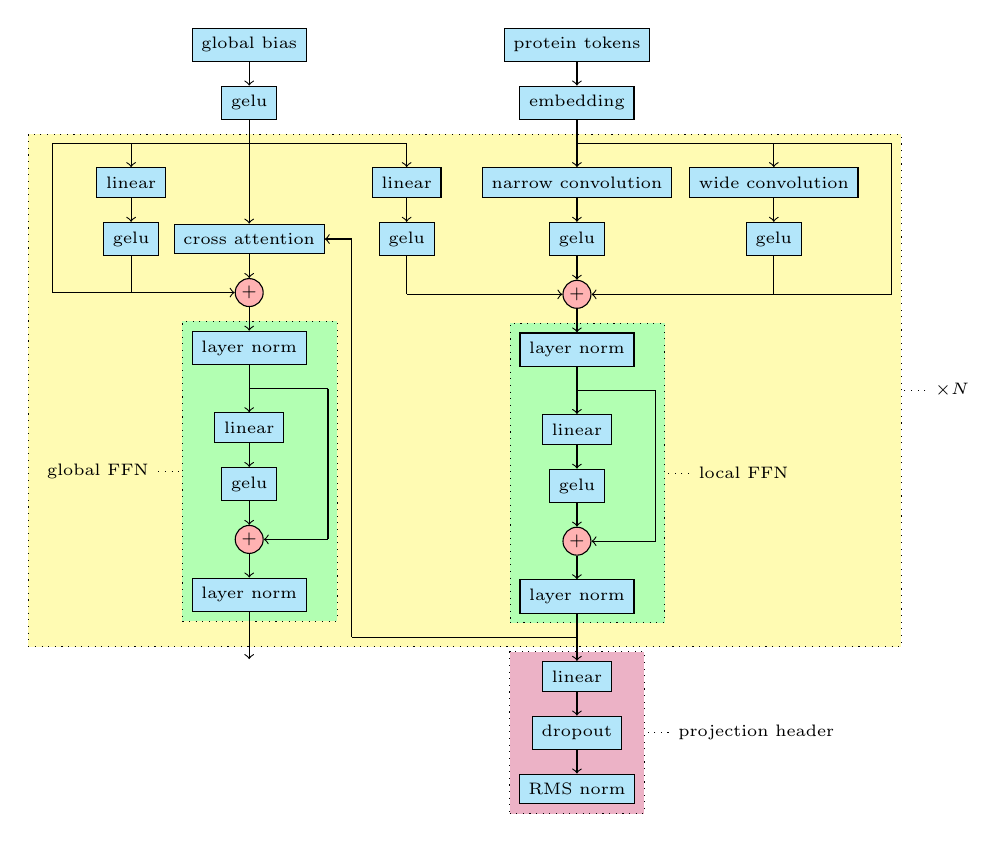
\begin{tikzpicture}
            \node[layer] (Token) {protein tokens};
            \node[layer] (Embed) [below=of Token] {embedding};
            \draw[->] (Token) -- (Embed);
            
            \coordinate[below=of Embed] (EmbedResidualStart);
            \draw[-] (Embed) -- (EmbedResidualStart);
            \node[layer] (NarrowConv) [below=of EmbedResidualStart] {narrow convolution};
            \draw[->] (EmbedResidualStart) -- (NarrowConv);
            \node[layer] (NarrowGelu) [below=of NarrowConv] {gelu};
            \draw[->] (NarrowConv) -- (NarrowGelu);
            \node[sum] (EmbedResidualEnd) [below=of NarrowGelu] {+};
            \draw[->] (NarrowGelu) -- (EmbedResidualEnd);

            \coordinate[right=2.5cm of EmbedResidualStart] (EmbedResidualBranch);
            \draw[-] (EmbedResidualStart) -- (EmbedResidualBranch);
            \node[layer] (WideConv) [below=of EmbedResidualBranch] {wide convolution};
            \draw[->] (EmbedResidualBranch) -- (WideConv);
            \node[layer] (WideGelu) at (NarrowGelu-|WideConv) {gelu};
            \draw[->] (WideConv) -- (WideGelu);
            \coordinate (WideGeluAnchor) at (EmbedResidualEnd-|WideGelu);
            \draw[-] (WideGelu) -- (WideGeluAnchor);
            \draw[->] (WideGeluAnchor) -- (EmbedResidualEnd);

            \coordinate[right=1.5cm of EmbedResidualBranch] (EmbedResidualTurn);
            \draw[-] (EmbedResidualBranch) -- (EmbedResidualTurn);
            \coordinate (EmbedResidualTurnAnchor) at (EmbedResidualEnd-|EmbedResidualTurn);
            \draw[-] (EmbedResidualTurn) -- (EmbedResidualTurnAnchor);
            \draw[-] (EmbedResidualTurnAnchor) -- (WideGeluAnchor);

            \node[layer] (GlobalBias) [left=2.5cm of Token] {global bias};
            \node[layer] (GlobalGelu) [below=of GlobalBias] {gelu};
            \draw[->] (GlobalBias) -- (GlobalGelu);
            \coordinate[below=of GlobalGelu] (GlobalResidualStart);
            \draw[-] (GlobalGelu) -- (GlobalResidualStart);
            \coordinate[right=2cm of GlobalResidualStart] (GlobalTokenTurn);
            \draw[-] (GlobalResidualStart) -- (GlobalTokenTurn);
            \node[layer] (GlobalLinear) [below=of GlobalTokenTurn] {linear};
            \draw[->] (GlobalTokenTurn) -- (GlobalLinear);
            \node[layer] (GlobalLinearGelu) [below=of GlobalLinear] {gelu};
            \draw[->] (GlobalLinear) -- (GlobalLinearGelu);
            \coordinate (GlobalLinearGeluAnchor) at (EmbedResidualEnd-|GlobalLinearGelu);
            \draw[-] (GlobalLinearGelu) -- (GlobalLinearGeluAnchor);
            \draw[->] (GlobalLinearGeluAnchor) -- (EmbedResidualEnd);

            \node[layer] (LocalFFNLayerNorm1) [below=of EmbedResidualEnd] {layer norm};
            \draw[->] (EmbedResidualEnd) -- (LocalFFNLayerNorm1);
            \coordinate[below=of LocalFFNLayerNorm1] (LocalFFNResidualStart);
            \draw[-] (LocalFFNLayerNorm1) -- (LocalFFNResidualStart);
            \node[layer] (LocalFFNLinear) [below=of LocalFFNResidualStart] {linear};
            \draw[->] (LocalFFNResidualStart) -- (LocalFFNLinear);
            \node[layer] (LocalFFNGelu) [below=of LocalFFNLinear] {gelu};
            \draw[->] (LocalFFNLinear) -- (LocalFFNGelu);
            \node[sum] (LocalFFNResidualEnd) [below=of LocalFFNGelu] {+};
            \draw[->] (LocalFFNGelu) -- (LocalFFNResidualEnd);
            \node[layer] (LocalFFNLayerNorm2) [below=of LocalFFNResidualEnd] {layer norm};
            \draw[->] (LocalFFNResidualEnd) -- (LocalFFNLayerNorm2);
            \coordinate[right=1cm of LocalFFNResidualStart] (LocalFFNResidualStartAnchor);
            \draw[-] (LocalFFNResidualStart) -- (LocalFFNResidualStartAnchor);
            \coordinate (LocalFFNResidualEndAnchor) at (LocalFFNResidualEnd-|LocalFFNResidualStartAnchor);
            \draw[-] (LocalFFNResidualStartAnchor) -- (LocalFFNResidualEndAnchor);
            \draw[->] (LocalFFNResidualEndAnchor) -- (LocalFFNResidualEnd);
            \coordinate[below=of LocalFFNLayerNorm2] (LocalBeforeOutput);
            \draw[-] (LocalFFNLayerNorm2) -- (LocalBeforeOutput);
            \begin{pgfonlayer}{background}
                \node[draw, dotted, fill=green!30, fit=(LocalFFNLayerNorm1)(LocalFFNResidualStart)(LocalFFNLinear)(LocalFFNGelu)(LocalFFNResidualEnd)(LocalFFNLayerNorm2)(LocalFFNResidualStartAnchor)(LocalFFNResidualEndAnchor)] (LocalFFNModule) {};
                \node[annot] (LocalFFNModuleName) [right=of LocalFFNModule] {local FFN};
                \draw[dotted] (LocalFFNModuleName) -- (LocalFFNModule);
            \end{pgfonlayer}

            \coordinate[below=of LocalFFNLayerNorm2] (TokenBranch);
            \draw[-] (LocalFFNLayerNorm2) -- (TokenBranch);
            \node[layer] (CrossAttention) at (GlobalLinearGelu-|GlobalResidualStart) {cross attention};
            \draw[->] (GlobalResidualStart) -- (CrossAttention);
            \coordinate (CrossAttentionToken) at ($ (CrossAttention.east)!1/2!(GlobalLinearGelu.west) $);
            \coordinate (CrossAttentionTokenAnchor) at (TokenBranch-|CrossAttentionToken);
            \draw[-] (TokenBranch) -- (CrossAttentionTokenAnchor);
            \draw[-] (CrossAttentionTokenAnchor) -- (CrossAttentionToken);
            \draw[->] (CrossAttentionToken) -> (CrossAttention);
            \node[sum] (GlobalResidualEnd) [below=of CrossAttention] {+};
            \draw[->] (CrossAttention) -- (GlobalResidualEnd);

            \node[layer] (GlobalFFNLayerNorm1) [below=of GlobalResidualEnd] {layer norm};
            \draw[->] (GlobalResidualEnd) -- (GlobalFFNLayerNorm1);
            \coordinate[below=of GlobalFFNLayerNorm1] (GlobalFFNResidualStart);
            \draw[-] (GlobalFFNLayerNorm1) -- (GlobalFFNResidualStart);
            \node[layer] (GlobalFFNLinear) [below=of GlobalFFNResidualStart] {linear};
            \draw[->] (GlobalFFNResidualStart) -- (GlobalFFNLinear);
            \node[layer] (GlobalFFNGelu) [below=of GlobalFFNLinear] {gelu};
            \draw[->] (GlobalFFNLinear) -- (GlobalFFNGelu);
            \node[sum] (GlobalFFNResidualEnd) [below=of GlobalFFNGelu] {+};
            \draw[->] (GlobalFFNGelu) -- (GlobalFFNResidualEnd);
            \node[layer] (GlobalFFNLayerNorm2) [below=of GlobalFFNResidualEnd] {layer norm};
            \draw[->] (GlobalFFNResidualEnd) -- (GlobalFFNLayerNorm2);
            \coordinate[right=1cm of GlobalFFNResidualStart] (GlobalFFNResidualStartAnchor);
            \draw[-] (GlobalFFNResidualStart) -- (GlobalFFNResidualStartAnchor);
            \coordinate (GlobalFFNResidualEndAnchor) at (GlobalFFNResidualEnd-|GlobalFFNResidualStartAnchor);
            \draw[-] (GlobalFFNResidualStartAnchor) -- (GlobalFFNResidualEndAnchor);
            \draw[->] (GlobalFFNResidualEndAnchor) -- (GlobalFFNResidualEnd);
            \coordinate[below=of GlobalFFNLayerNorm2] (GlobalBeforeOutput);
            \draw[-] (GlobalFFNLayerNorm2) -- (GlobalBeforeOutput);
            \coordinate[below=of GlobalBeforeOutput] (GlobalOutput);
            \draw[->] (GlobalBeforeOutput) -- (GlobalOutput);
            \begin{pgfonlayer}{background}
                \node[draw, dotted, fill=green!30, fit=(GlobalFFNLayerNorm1)(GlobalFFNResidualStart)(GlobalFFNLinear)(GlobalFFNGelu)(GlobalFFNResidualEnd)(GlobalFFNLayerNorm2)(GlobalFFNResidualStartAnchor)(GlobalFFNResidualEndAnchor)] (GlobalFFNModule) {};
                \node[annot] (GlobalFFNModuleName) [left=of GlobalFFNModule] {global FFN};
                \draw[dotted] (GlobalFFNModuleName) -- (GlobalFFNModule);
            \end{pgfonlayer}
            
            \coordinate[left=1.5cm of GlobalResidualStart] (GlobalResidualBranch);
            \draw[-] (GlobalResidualStart) -- (GlobalResidualBranch);
            \node[layer] (GlobalLinear2) [below=of GlobalResidualBranch] {linear};
            \draw[->] (GlobalResidualBranch) -- (GlobalLinear2);
            \node[layer] (GlobalLinearGelu2) [below=of GlobalLinear2] {gelu};
            \draw[->] (GlobalLinear2) -- (GlobalLinearGelu2);
            \coordinate (GlobalResidualBranchAnchor) at (GlobalResidualEnd-|GlobalLinearGelu2);
            \draw[-] (GlobalLinearGelu2) -- (GlobalResidualBranchAnchor);
            \draw[->] (GlobalResidualBranchAnchor) -- (GlobalResidualEnd);

            \coordinate[left=1cm of GlobalResidualBranch] (GlobalResidualTurn);
            \draw[-] (GlobalResidualBranch) -- (GlobalResidualTurn);
            \coordinate (GlobalResidualTurnAnchor) at (GlobalResidualBranchAnchor-|GlobalResidualTurn);
            \draw[-] (GlobalResidualTurn) -- (GlobalResidualTurnAnchor);
            \draw[-] (GlobalResidualTurnAnchor) -- (GlobalResidualBranchAnchor);

            \begin{pgfonlayer}{backbackground}
                \node[draw, dotted, fill=yellow!30, fit=(NarrowConv)(NarrowGelu)(EmbedResidualEnd)(EmbedResidualStart)(EmbedResidualBranch)(WideConv)(WideGelu)(WideGeluAnchor)(EmbedResidualTurn)(EmbedResidualTurnAnchor)(GlobalResidualStart)(GlobalTokenTurn)(GlobalLinear)(GlobalLinearGelu)(GlobalLinearGeluAnchor)(CrossAttention)(CrossAttentionToken)(GlobalResidualEnd)(GlobalResidualBranch)(GlobalLinear2)(GlobalLinearGelu2)(GlobalResidualEnd)(GlobalResidualTurn)(GlobalResidualTurnAnchor)(LocalFFNModule)(LocalFFNModuleName)(GlobalFFNModule)(GlobalFFNModuleName)(LocalBeforeOutput)(GlobalBeforeOutput)(CrossAttentionTokenAnchor)] (LocalGlobalModule) {};
                \node[annot] (LocalGlobalModuleName) [right=of LocalGlobalModule] {$\times N$};
                \draw[dotted] (LocalGlobalModuleName) -- (LocalGlobalModule);
            \end{pgfonlayer}

            \node[layer] (PBHLinear) [below=of LocalBeforeOutput] {linear};
            \draw[->] (LocalBeforeOutput) -- (PBHLinear);
            \node[layer] (PBHDrop) [below=of PBHLinear] {dropout};
            \draw[->] (PBHLinear) -- (PBHDrop);
            \node[layer] (PBHNormRMS) [below=of PBHDrop] {RMS norm};
            \draw[->] (PBHDrop) -- (PBHNormRMS);
            \begin{pgfonlayer}{background}
                \node[draw, dotted, fill=purple!30, fit=(PBHLinear)(PBHDrop)(PBHNormRMS)] (PBHModule) {};
                \node[annot] (PBHModuleName) [right=of PBHModule] {projection header};
                \draw[dotted] (PBHModuleName) -- (PBHModule);
            \end{pgfonlayer}
        \end{tikzpicture}
    }
    \caption{The architecture of protein bert. The model takes redidue-wise information and global protein information. The redidue-wise information is processed by narrow and wide convolutions, which replaces attention mechanism. The cross attention is a strandard one, but between the single global embedding and the multiple residue embeddings. Thus, the complexity is linear with the length of the protein. Also, the information flow between the local and global representations allows residues depend on each other through the cross attention. The projection header is added to make the output dimention consistent with our model.}\label{fig:protein_bert_architecture}
\end{figure}

\subsubsection{The secondary structure encoder}
The secondary structure is encoded by a strand transformer encoder structure repeated by several times. The normalized output embedding is used for cross-attention with DNA embeddings.

\begin{figure}[H]
    \centering
    \makebox[0pt]{
        \hspace*{0cm}

        \begin{tikzpicture}
            \node[layer] (Token) {secondary tokens};
            \node[layer] (Embed) [below=of Token] {embedding};
            \draw[->] (Token) -- (Embed);
            \node[layer] (Drop) [below=of Embed] {dropout};
            \draw[->] (Embed) -- (Drop);

            \coordinate[below=of Drop] (SelfResidualStart);
            \draw[-] (Drop) -- (SelfResidualStart);
            \node[layer] (SelfNormRMS) [below=of SelfResidualStart] {RMS norm};
            \draw[->] (SelfResidualStart) -- (SelfNormRMS);
            \node[layer] (SelfAttention) [below=of SelfNormRMS] {self attention};
            \draw[->] (SelfNormRMS) -- (SelfAttention);
            \node[sum] (SelfResidualEnd) [below=of SelfAttention] {$+$};
            \draw[->] (SelfAttention) -- (SelfResidualEnd);

            \coordinate[left=1.5cm of SelfResidualStart.center] (SelfResidualStartAnchor);
            \coordinate[left=1.5cm of SelfResidualEnd.center] (SelfResidualEndAnchor);
            \draw[-] (SelfResidualStart) -- (SelfResidualStartAnchor);
            \draw[-] (SelfResidualStartAnchor) -- (SelfResidualEndAnchor);
            \draw[->] (SelfResidualEndAnchor) -- (SelfResidualEnd);

            \begin{pgfonlayer}{background}
                \node[draw, dotted, fill=green!30, fit=(SelfResidualStart)(SelfNormRMS)(SelfAttention)(SelfResidualEnd)(SelfResidualStartAnchor)(SelfResidualEndAnchor)] (SelfModule) {};
                \node[annot] (SelfModuleName) [right=of SelfModule] {attention};
                \draw[dotted] (SelfModuleName) -- (SelfModule);
            \end{pgfonlayer}

            \coordinate[below=of SelfResidualEnd] (FFNResidualStart);
            \draw[-] (SecondResidualEnd) -- (FFNResidualStart);
            \node[layer] (FNNNormRMS) [below=of FFNResidualStart] {RMS norm};
            \draw[->] (FFNResidualStart) -- (FNNNormRMS);
            \node[layer] (FFNLinear1) [below=of FNNNormRMS] {linear};
            \draw[->] (FNNNormRMS) -- (FFNLinear1);
            \node[layer] (FFNGelu) [below=of FFNLinear1] {gelu};
            \draw[->] (FFNLinear1) -- (FFNGelu);
            \node[layer] (FFNLinear2) [below=of FFNGelu] {linear};
            \draw[->] (FFNGelu) -- (FFNLinear2);
            \node[layer] (FFNDrop) [below=of FFNLinear2] {dropout};
            \draw[->] (FFNLinear2) -- (FFNDrop);
            \node[sum] (FFNResidualEnd) [below=of FFNDrop] {+};
            \draw[->] (FFNDrop) -- (FFNResidualEnd);

            \coordinate[left=1cm of FFNResidualStart.center] (FFNResidualStartAnchor);
            \coordinate[left=1cm of FFNResidualEnd.center] (FFNResidualEndAnchor);
            \draw[-] (FFNResidualStart) -- (FFNResidualStartAnchor);
            \draw[-] (FFNResidualStartAnchor) -- (FFNResidualEndAnchor);
            \draw[->] (FFNResidualEndAnchor) -- (FFNResidualEnd);

            \begin{pgfonlayer}{background}
                \node[draw, dotted, fill=green!30, fit=(FFNResidualStart)(FNNNormRMS)(FFNLinear1)(FFNGelu)(FFNLinear2)(FFNDrop)(FFNResidualEnd)(FFNResidualStartAnchor)(FFNResidualEndAnchor)] (FFNModule) {};
                \node[annot] (FFNModuleName) [right=of FFNModule] {FFN};
                \draw[dotted] (FFNModuleName) -- (FFNModule);
            \end{pgfonlayer}

            \begin{pgfonlayer}{backbackground}
                \node[draw, dotted, fill=yellow!30, fit=(SelfModule)(SelfModuleName)(FFNModule)(FFNModuleName)] (Repeats) {};
                \node[annot] (RepeatsTimesN) [right=of Repeats] {$\times N$};
                \draw[dotted] (RepeatsTimesN) -- (Repeats);
            \end{pgfonlayer}

            \node[layer] (LastNormRms) [below=of FFNResidualEnd] {RMS norm};
            \draw[->] (FFNResidualEnd) -> (LastNormRms);
        \end{tikzpicture}
    }
    \caption{The architecture of secondary structure encoder. This is a quite standard transformer structure. We resemble DeepSeek to use RMS normalization instead of layer normalization, and move RMS normalization before the attention module.}\label{fig:secondary_architecture}
\end{figure}

\subsection{Positive and negative samples}
There are 62 C2H2 zinc finger protein, each with 3000 randomly seleted binding sites, thereby $62\times 3000$ binding sites. Each pair of protein and binding site forms a sample. There are totally $62\times 62\times 3000$ pairs, among which $62\times 3000$ are positive samples (protein and binding site are matched), and $61\times 62\times 3000$ are negative samples (protein and binding site are unmatched). The samples are quite imbalance because there are many more negative samples than positive ones. Resampling and class-balanced focal loss are two common way to solve the resampling problem. However, both methods need train on all negative samples, which is very time-consuming. A workaround is to downsample negative samples to the same number of postive ones. The lightGBM propose gradient-based one-side sampling (GOSS) to select sample based on the loss\cite{NIPS2017_6449f44a}. We accept this strategy to select hard negative samples with large loss.

In detail, for each binding site (i.e. DNA) in a batch, we use their corresponding C2H2 zinc finger protein to form positive samples. The number of positive samples in a batch is thus exactly the batch size $B$. Then we select $B$ negative samples from the totally $B\times 61$ negative samples in the batch as follows. We first exclude the negative sample that the non-corresponding C2H2 zinc finger protein binding within a certain distance (300bp in our setting) to the current binding site. For the remaining negative samples, we sort them according to their loss recorded in previous training epochs. We choose a certain ratio $R$ (50\% in our setting), and select $B\times R$ of negative samples with the largest loss. These are hard negative samples and can help to improve the model performance. Then we randomly select $B\times (1-R)$ negative samples without replacement from the remaining negative samples. We do not select all negative samples based on loss because it will break the internal distribution of the negative samples.

\subsection{Benchmarks}
We compare our models with lightGBM and some classic machine learning classifiers including support vector machine with stochastic gradient descent (SGD) learning, perceptron, passive aggressive, decision tree, random forest, AdaBoost, naive bayes. We also include a dummy classifer as control which does not use the information of inputs (i.e. DNA, protein, secondary structure). To fit the data into memory, we downsample the negative samples to the same length of the positive samples. We concatenate the tokenized DNA, protein and secondary structure as input features to these models.

The results are illustrated in Table \ref{tab:benchmarks}. Methods based on ensemble learning, i.e. lightGBM and AdaBoost based on boosting, Random Forest based on bootstrap aggregating (also called bagging), have higher accuracies than those of other common machine learning methods. Compare with $0.497$ of the dummy classifier (control), those ensembling learning based methods have accuracies around $0.59$. Other methods have accuracy slightly higher than the control value $0.497$. The Naive Bayes performances better than linear methods, i.e. SVM, perceptron, passive aggressive, which implies that the binding problem of C2H2 zinc finger has non-linear nature.
\begin{table}[H]
    \caption{Performances of lightGBM, common machine learning classifiers and DeepZF.}\label{tab:benchmarks}
    \begin{tabular}{|l|l|l|l|l|l|l|l|l|l|}
        \hline
        algorithm & f1 & accuracy & recall & precision & matthews correlation \\
        \hline
        lightGBM & 0.522 & 0.594 & 0.443 & 0.635 & 0.197 \\
        SVM & 0.114 & 0.522 & 0.062 & 0.769 & 0.110 \\
        Perceptron & 0.093 & 0.520 & 0.049 & 0.846 & 0.120 \\
        Passive Aggressive & 0.030 & 0.507 & 0.015 & 0.906 & 0.075 \\
        Decision Tree & 0.530 & 0.525 & 0.534 & 0.525 & 0.051 \\
        Random Forest & 0.538 & 0.586 & 0.482 & 0.609 & 0.176 \\
        AdaBoost & 0.524 & 0.592 & 0.449 & 0.629 & 0.193 \\
        Naive Bayes & 0.521 & 0.539 & 0.501 & 0.543 & 0.079 \\
        Dummy & 0.497 & 0.497 & 0.497 & 0.497 & -0.007 \\
        DeepZF & 0.621 & 0.514 & 0.794 & 0.509 & 0.035 \\
        \hline
    \end{tabular}
\end{table}

We also test a previously proposed deep learning model DeepZF \cite{10.1093/bioinformatics/btac469}. DeepZF consists of two parts. The first part classifies C2H2 zinc fingers into those binding DNA triplet and those not binding DNA. It predicts a binding probability for the C2H2 zinc finger based on its context sequence. The second part of DeepZF predict a triplet DNA binding motif for a C2H2 zinc finger. The triplet DNA motif of all tandom C2H2 zinc finger predicted to bind DNA are concatenate in order to get the binding motif of the protein. We apply DeepZF to all 62 C2H2 zinc finger proteins in our data set to get 62 motifs. Then we use fimo to calculate the motif scores in negative and positive bind sites. A score threshold is needed to determine whether a give site binding the protein of the motif. We select the best score threshold based on 90\% data, and apply the threshold to the remaining 10\% data to evaluate its performance in predicting binding sites. The results is given in Table \ref{tab:benchmarks}. DeepZF does not outperformance those common machine learning classifiers.

\bibliographystyle{plain}
\bibliography{reference.bib}

\end{document}